\chapter{Problemløsning}
I dette kapitel vil gruppen beskrive hvilke krav gruppen stiller til projektet, hvilke teorier og algoritmer der er vigtige i forhold til projektet og hvordan gruppen har valgt at lave programmet, altså implementeringsprocessen.

\section{Kravspecifikationer}
I dette afsnit vil gruppen vurdere, hvilke krav der skal indegå i en løsning. Heri vil der både blive opstillet krav til en optimal løsning og til en afgrænset løsning, som gruppen mener at være realistisk, at kunne lave.

\subsection{Optimale løsningsforslag}
For at kunne udvilke en softwareløsning, der besvarer gruppens problemformulering, er det vigtigt at definere nogle krav til programmet. Til en optimal løsning, har gruppen vurderet, at der skal være følgende krav:
\begin{itemize}
	\item Programmet skal udvikles som en applikation til moderne smartphones, inklusiv iOS, Android og Windows Phone.
	\item Programmet skal hjælpe brugeren, til at lave en interresant rute gennem byen vedkommende vil besøge.
	\item Programmet skal vise et overskueligt og scalerbart kort med ruten.
	\item Ruten skal udskrives i samme stil som Google Maps.
	\item Programmet skal kunne give rutevejledning undervejs på ruten. 
	\item Programmet skal kunne  downloade en offline version af den rute der er valgt, inklusiv kortet for det omkringliggende område.
\end{itemize}
Til disse krav har gruppen konstrueret nogle skitser og en beskrivelse af den optimale løsning, for at give et billede af hvordan det eventuelt kunne se ud. \newpage

Gruppen har valgt at lave den ideele løsning på følgende måde:\newline
\newline
Brugeren bliver præsenteret for en liste over alle attraktioner i byen, sorteret efter afstand fra brugerens nuværende position, alfabetisk rækkefølge eller rating. \newline
Ratingen vil blive fundet ved at tage gennemsnittet af alle brugeres rating af den specifikke attraktion. \newline
Dette gøres for at give brugeren mulighed for at vælge de attraktioner vedkommende gerne vil se.\newline
\newline
Programmet skal under udvælgelsen give brugeren mulighed for at læse om de enkelte attraktioner, så brugeren kan foretage indformerede beslutninger om til og fravælgelse af attraktioner.\newline
\newline
Når brugeren har valgt de attraktioner vedkommende vil besøge, udformes et kort med den korteste rute mellem disse attraktioner. På dette kort vil alle attraktioner som ligger indefor en forudbestemt afstand til ruten, blive vist. Derefter kan brugeren tilføje nogle ekstra attraktioner, som vil blive tilføjet til den endelige rute.\newline
Dette gøres så brugeren kan udforme en mere interessant rute. Gruppen vil ikke diktere hvad den interessante rute er, men lade brugeren selv tilvælge, og derved få deres egen unikke interresante rute. \newline 
 

\begin{wrapfigure}{r}{0.3\textwidth}
  \vspace{-20pt}
  \begin{center}
    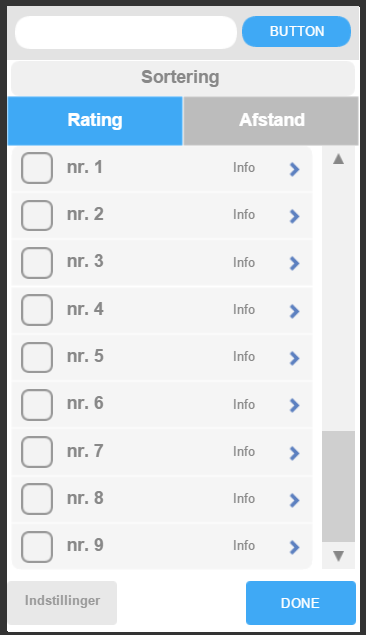
\includegraphics[scale=0.35]{start1} \newline
    \textit{Figur 3.1: Brugergrænseflade}\newline
  \end{center}
  \vspace{-20pt}
  \vspace{-20pt}
\end{wrapfigure}


Gruppen ønsker, at programmet skulle fungere på den måde, at der findes to valg muligheder, forholdsvis rating og afstand, hvoraf rating viser en række attraktioner med en værdi, baseret på hvad brugerne har valgt at rate den. Funktionen afstand, vil vise hvor stor en afstand der er fra det punkt hvor brugeren står, til en attraktion. De attraktioner, som brugeren ønsker at se, skal brugeren blot tjekke af, ved at klikke på attraktionerne, og de vil derefter blive tilføjet til den nuværende rute. Figur 3.1 viser en skitse af brugergrænsefladen. \newline
\newline
\newline
\newline

\begin{wrapfigure}{l}{0.3\textwidth}
  \vspace{-50pt}
  \begin{center}
    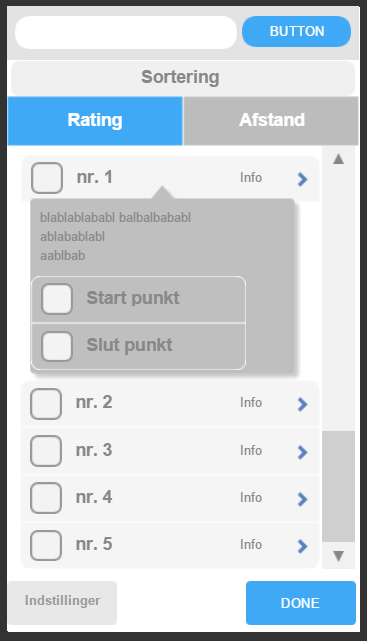
\includegraphics[scale=0.35]{start2} \newline
    \textit{Figur 3.2: \newline Udvidet brugergrænseflade}\newline
  \end{center}
  \vspace{20pt}
\end{wrapfigure}

Herudover ønsker gruppen, at der er en form for menu, som indeholder informationer omkring de forskellige attraktioner. Udover dette, skal der også være mulighed for at vælge et start- eller slutpunkt. Disse punkter skal give brugeren mulighed for at vælge, hvor brugeren ønsker at starte/slutte sin rute. Figur 3.2 viser en skitse af en udvidet brugergrænseflade.\newline
\newline
\newline
\newline
\newline

\begin{wrapfigure}{r}{0.3\textwidth}
  \vspace{-30pt}
  \begin{center}
    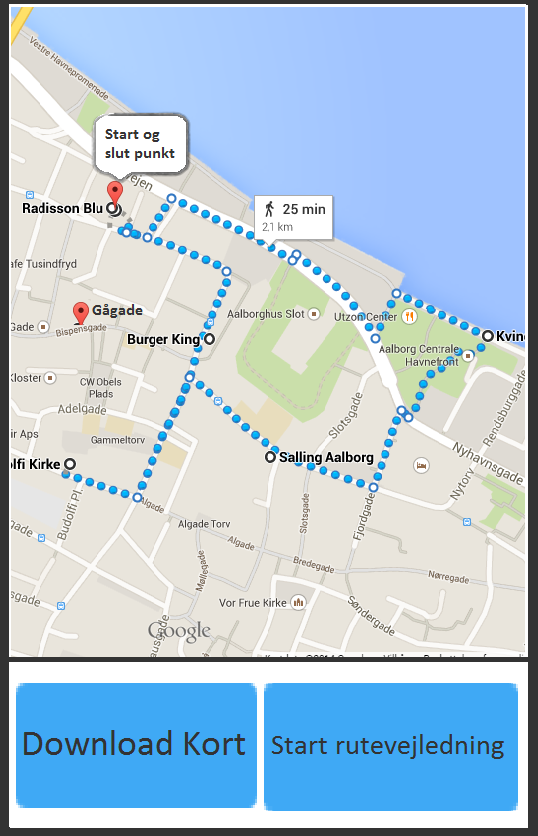
\includegraphics[scale=0.3]{rute1} \newline
    \textit{Figur 3.3: Rute - Ruten er\newline hentet fra Maps.Google.com}\newline
  \end{center}
  \vspace{0pt}
  \vspace{-100pt}
\end{wrapfigure}


Når der er valgt nogle ønskede destinationer/attraktioner, skal programmet fremvise en rute. Ruten skal vise hvor lang hele ruten er, og hvor lang tid det tager at gå ruten. Der skal desuden være to funktioner, når ruten bliver vist. Der skal være mulighed for at downloade kortet på mobilen, og derved gør det muligt at anvende programmet, uden brug af internet. Den anden funktion skal starte rutevejledningen, som fungere som en ganske almindelig GPS. En skitse af dette kan ses på figur 3.3.
\newpage

\begin{wrapfigure}{r}{0.3\textwidth}
  \vspace{-20pt}
  \begin{center}
    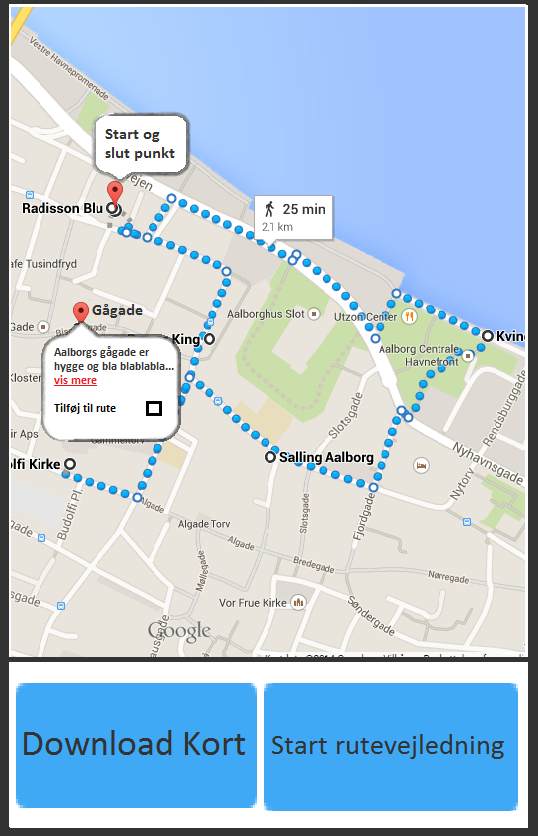
\includegraphics[scale=0.3]{rute2} \newline
    \textit{Figur 3.4: Udvidet rute - Ruten er hentet fra\newline Maps.Google.com}\newline
  \end{center}
  \vspace{-20pt}
  \vspace{-10pt}
\end{wrapfigure}

Der skal desuden også her være mulighed for at få information om attraktionerne, der er i nærheden af den valgte rute. Der skal være en "tilføj til nuværende rute"-funktion, som tilføjer de valgte attraktioner, som er i nærheden til den rute, der allerede er lavet. Figur 3.4 viser hvordan det eventuelt kunne laves. \newline
\newline
\newline
\newline
\newline
\newline
\newline
\newline
\newline
 

\subsection{Gruppens løsningsforslag}
Gruppen har gennem spørgskema og interview, fået stillet en række krav til løsningen, af turister og VisitAalborg. 
Gennem spørgskemaet, blev det konkluderet, at det vigtigste for turister, er at de kan opleve byen på en interessant rute. 
Derudover har turistbureauet givet udtryk for, at løsningen gerne skal være så enkelt som muligt, altså meget få funktioner, så brugeren ikke bliver forvirret, da de mener, at det er i turistens bedste interesse. \newline
Der er blevet stillet krav fra universitets side, om at programmet skal være et lille specifikt program i C, af høj kvalitet. Dette stemmer godt overens, med de krav der er blevet stillet fra turistbureauets side.   \newline
Ud fra dette, har gruppen opsat nogle krav for gruppens løsningsforslag, og de er som følgende:
\begin{itemize}
	\item Programmet skal kunne beregne den korteste rute mellem en række punkter.
	\item Programmet skal give beregne om der ligger en attraktion tæt ved ruten, og tilføje ekstra attraktionen til ruten.
 	\item Programmet skal som output, give en liste over rutens destinationer.
\end{itemize}

Da dette er et P1 projekt, og gruppen er begrænset af både tid og erfaring, har gruppen valgt at begrænse softwareløsningen, på følgende punkter: 
\begin{itemize}
	\item Rutevejledningen bliver i fugleflugtslinje.
	\item Brugeren kan kun vælge destinationer ud fra en række forudbestemte punkter.
	\item Tekstbaseret brugergrænseflade.
\end{itemize}

På baggrund af kravene og afgrænsningen, har gruppen tænkt sig at lave et program, som har nogle forudbestemte destinationer, der dækker over destinationerne i Aalborg, hvorefter brugeren vælger de destinationer han/hun ønsker at besøge. Programmet vil ud fra disse punkter, beregne den korteste rute, og undersøge om der er andre attraktioner, som ligger tæt på ruten, og spørge brugeren, om det kunne være interessant at besøge disse steder. Hvis ja, vil disse punkter også blive inkluderet. På den måde for brugeren selv lov til at skabe sig den mest interresante rute. Resultatet bliver en liste over destinationerne, der står i rækkefølge, så turisten ved hvilken rækkefølge de skal besøge dem i, for at få den mest optimale rute.

\section{Teorier}
Indledning mangler.

\subsection{Grafteori}
Grafteori er et afsnit i denne rapport, som omhandler en generel forklaring på graf teori, hvorefter teorien bag ”Nærmeste Nabo Algoritme” vil blive beskrevet, herefter forklares ”udregningstid” i rute-algoritmer, og til sidst Traveling Salesman Problem. Alt dette beskrives, for at give et udgangspunkt for implementering af en hensigtsmæssig algoritme i programmet for denne rapport.\newline
Matematikken bag graf teori er ét aspekt af emnet, hvor visualisering og tegning er en anden. Den matematiske del behandler kombinationerne af knuder og kanter. En knude er et punkt, i vores tilfælde en attraktion som skal besøges, hvor en kant er vejen derhen. En kant er derfor længden fra ét punkt til det næste \citep{GraphTheory}.
I graf teori er begrebet ”graf” mere fleksibelt, da punkterne ikke nødvendigvis har x, y eller z værdier, alt efter antallet af dimensioner man behandler det i. Grafen i denne form er en afbildning af punkter i den form, hvor det virker hensigtsmæssigt. Heraf opstår isomorfiske modeller, som er forskellige afbildninger, af selv samme graf. 

\begin{wrapfigure}{}{0.6\textwidth}
  \vspace{-20pt}
  \begin{center}
    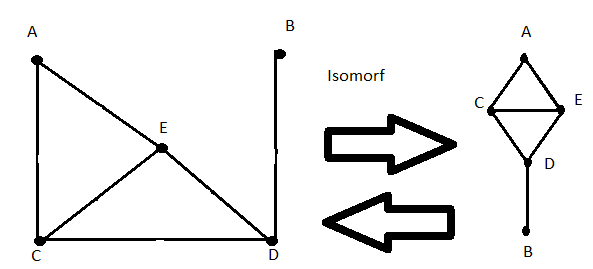
\includegraphics[scale=0.8]{grafteori1} \newline
    \textit{Figur 5.1: Brugergrænseflade}\newline
  \end{center}
  \vspace{-20pt}
  \vspace{-20pt}
\end{wrapfigure}

Denne matematik-type er stadig under udforskning, da der endnu ikke er en fuldstændig løsning på problemer i teorien, for blandt andet ”Traveling Salesman Problem”. Heriblandt findes mange typer af problemer, hvor forskellige teoretiske løsninger kan bruges. 
En af problematikkerne vedrørende Traveling Salesman Problem er, at der ønskes både en optimal rute, og en udregningstid der er hensigtsmæssig. Dette problem opstår i det, at en optimal rute skal findes mellem et hvis antal byer (knuder), hvor man i ét kan lave en hurtig estimeret ”kort” rute, hvis man starter med at lave tilfældige kanter fra knuderne, dog ikke mere end to kanter per knude, og derefter tester for, hvorvidt to nye kanter er kortere end to eksisterende kanter. På et tidspunkt vil en semi-optimal rute findes, dog er denne ikke nødvendigvis den fuldt optimale rute. Dette skyldes, at der igennem forløbet med udskiftning af kanter muligvis er truffet valg om rute som fører til, at en kortere kant ikke kan findes lokalt, men at den sammenlagte rute stadig ikke er optimal. Hvis der er fundet korte kanter lokalt, kan dette stoppe søgen i en kortere kant, da den korteste lokale kant er fundet, men ikke den korteste kant, hvis der tages hensyn til den sammenlagte kant-værdi. \citep{TSP}
\newline

\textbf{Nearest Neighbor Algoritme}\newline
En af disse løsninger er den Nærmeste Nabo Algoritme (NNA, Nearest Neighbor Algorithm), som behandler et problem der opstår, når en række knuder skal indgå, og kun skal indgå én gang, hvilket betyder, at der ikke må være en løkke (loop). Dette opnåes gennem brug af Hamiltonian Paths, hvilket er en ”rute” gennem knuder på grafen. I NAA vil en kant have en værdi, og disse værdier er bestemmende for, hvilken kant der skal følges. Fra den knude der behandles, skal kanten med den laveste værdi følges. Dette kan dog optimeres, ved at lave en matrice over kanterne fra alle knuder. Her tages højde for hvilke kanter der samlet set giver den korteste rute, uden brug af løkker. \citep{NNA}
\newline

 
\begin{wrapfigure}{}{0.4\textwidth}
  \vspace{-40pt}
  \begin{center}
    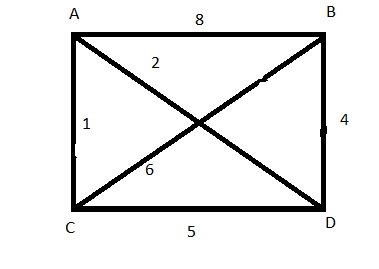
\includegraphics[scale=0.8]{grafteori2} \newline
    \textit{ Figur 4.2: Hamiltonian Path. \newline Følger kanter med laveste værdier.}
  \end{center}
  \vspace{-10pt}
\end{wrapfigure}

I dette tilfælde (figur 4.2), er den endelige rutes længde: 1+5+4+8 = 18. Spørgsmålet er så, er dette den koreste rute? Herefter opstilles en matrice, der beskriver alle kanter.

\begin{tabular}{| l | l | l | l | l | l |}
	\hline
	  & A & B & C & D & E \\ \hline
	A & - & 3 & 1 & - & 2 \\ \hline
	B & 3 & - & - & 3 & 8 \\ \hline
	C & 1 & - & - & 5 & 6 \\ \hline
	D & - & 4 & 5 & - & 7 \\ \hline
	E & 2 & 8 & 6 & 7 & - \\
	\hline
	\end{tabular}\newline
	

De mulige ruter er: \newline
ABDCE = 3+4+5+6 = 18. \newline
ACDBE = 1+5+4+8 = 18. \newline
AEBDC = 2+8+4+5 = 19. \newline
ABECD = 3+8+6+5 = 22. \newline
ABEDC = 3+8+7+5 = 23. \newline
ACEBD = 1+6+8+4 = 19. \newline
ACEDB = 1+6+7+4 = 18. \newline
AECDB = 2+6+5+4 = 17. \newline

Den korteste rute er altså AECDB, hvilket er 1 kortere end den antagede rute. Den optimale Hamiltonian Path er derfor denne rute. Dette tager NNA ikke højde for, da den starter i en valgt start-knude, og derefter følger kanten, med den derfra laveste værdi. Det smarte ved NNA er, at den ikke kræver meget kraft for en computer at udføre, hvorimod at finde den optimale Hamiltonian rute, vil være langt mere compliceret. NNA tager dog ikke højde for, hvad konsekvenser de skridt den tager, har for det endelige resultat.

\textbf{Dijkstra's algoritme}\newline
Udover NNA, findes også Dijkstra’s algoritme, hvor første step er, at bestemme ende-knuden, og sætte dens distance til nul. Denne knude sættes til at være den første knude, som behandles. I det en knude er checket færdig, vil denne knude markeres som ”besøgt”, og kanten med den mindste værdi følges, og næste knude markeres som ”nuværende” knude. En kant bliver kun fulgt, hvis det er den korteste rute, tilregnet tidligere kanter.
Problematikken med Dijkstra’s algoritme i forhold til dette projekt er, at den checker den korteste rute fra start-knude til slut-knude, men den indkluderer ikke nødvendigvis alle knuder som oplyses. I det denne rapport er afgrænset til fugleflugtslinjer, vil Dijkstra’s ikke være den optimale. Hvis en rute igennem en by, hvor der er tilregnet veje, stier og andre knuder, vil Dijkstra’s være det bedste valg. Denne algoritme vil også være i brug ved den optimale løsning. Ved brug af Dijkstra’s algoritme, vil den nuværende rute altid blive testet for, hvorvidt ruten der undersøges efter, er kortere eller længere end den hidtil korteste rute. Hvis den er kortere, vil denne rute blive sat som den hidtil korteste rute.\citep{Dijkstra}

\subsection{Vektorteori}
Essensen i dette projekt er at finde en flerpunktsrute mellem nogle valgte attraktioner, hvor brugeren skal have mulighed for, at vælge nogle attraktioner til deres rute. Gruppen vil ikke diktere hvad en interessant rute er for brugeren, derfor skal de have muligheden for at vælge de foreslåede attraktioner til eller fra.

\begin{wrapfigure}{}{0.4\textwidth}
  \vspace{-10pt}
  \begin{center}
    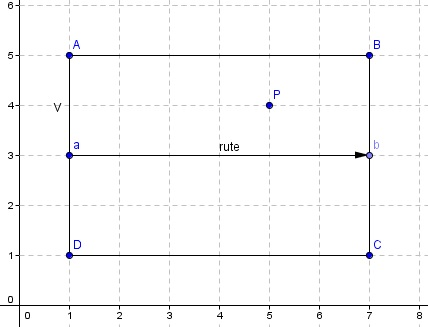
\includegraphics[scale=0.6]{matematikteori1} \newline
    \textit{Figur 5.1: Eksempel på om en attraktion er indenfor punkt a og b.}\newline
  \end{center}
  \vspace{-20pt}
\end{wrapfigure}
 
Der tages nu udgangspunkt i figur 5.1. En del af brugerens rute ligger fra attraktion a til attraktion b. Der skal nu tjekkes om der ligger andre attraktioner mellem afstanden fra a til b (eller AB), og med bredden AD hvor brugeren vil blive spurgt om denne attraktion skal tilføjes til ruten. AD er i projektets program sat til at være V * 2. Dette vil blive udregnet vha. vektorer 
Hvis der antages at punktet P er en attraktion som programmet skal tjekke, ligger denne inden for længden af ruten AB og bredden AD. Dette tjekkes med følgende formel:
\[0 < AP \cdot AB < AB \cdot AB \wedge 0 < AP \cdot AD < AD \cdot AD \]
Hvor prikproduktet af vektorerne AP og AB, skal være større end 0 og mindre end prikproduktet af vektorerne AB og AB. Det samme vil gælde for AD i stedet for AB.

Lad nu som om det de informationer der kendes er punkterne a og b, samt længden på vektor ab som vil være 6 og vektoren vil hedde:
\[ \begin{bmatrix} 6 \\ 0 \end{bmatrix} \]

Først ønskes punktet A findes, som gøres ved først at finde tværvektoren. Tværvektoren findes ved at bytte 1. og 2. koordinat rund og ændre fortegn på første koordinaten:
\[ \begin{matrix} a1 \\ a2 \end{matrix} = \begin{matrix} -a2 \\ a1 \end{matrix} \]
Tværvektoren hedder: 
\[ \begin{bmatrix} 6 \\ 0 \end{bmatrix} \text{ ,} \]
og har udgangs punkt fra punktet a. \newline
I dette eksempel skal der søges efter ekstra attraktioner langs ruten, svarende til 1/3 af rutens længde. Så for at finde koordinaterne til punktet A, finder vi først en enhedsvektor for tværvektoren, dette gøres med formlen:
\[ \overrightarrow{e} = \frac{1}{\overrightarrow{a}}*\overrightarrow{a} \] 

Dette giver en vektor: 
\[\ \begin{bmatrix} 0 \\ 1 \end{bmatrix} \text{ ,} \]
som også har udgangspunkt fra punktet a. Som tidligere nævnt søges der efter ekstra attraktioner langs ruten, svarende til 1/3 af rutens længde, så enhedsvektoren multipliceres med to, hvilket giver en vektor: 
\[\ \begin{bmatrix} 0 \\ 2 \end{bmatrix} \textbf{ .} \]
Denne vektor lægges til koordinaterne til punktet a, hvilket vil give punktet:
\[\ A = \begin{bmatrix} 1 \\ 3 \end{bmatrix} + \begin{bmatrix} 0 \\ 2 \end{bmatrix} = \begin{bmatrix} 1 \\ 5 \end{bmatrix} \text{ .} \]

Punktet D vil så ledes findes  ved at tage vektoren fra før og multiplicere med -2 og lægge punktet A til:
\[\ D = \begin{bmatrix} 0 \\ 2 \end{bmatrix} * -2 = \begin{bmatrix} 0 \\ -4 \end{bmatrix} + \begin{bmatrix} 1 \\ 5 \end{bmatrix} = \begin{bmatrix} 1 \\ 1 \end{bmatrix} \text{ .} \]



Dog vil der først findes en vektor AP mellem punkterne A og P med formlen: \[ \overrightarrow{AP} = \begin{matrix}X2-X1 \\ Y2-Y1\end{matrix} \]
Vektor AP: A(1,5) og P(5,4): \[ \overrightarrow{AP} = \begin{bmatrix}5-1 \\ 4-5\end{bmatrix} = \begin{bmatrix} 4 \\ -1 \end{bmatrix} \]
\[ \text{Vektor AB er allerede kendt, da det er det samme som } \overrightarrow{ab} \text{.} \]
For at projektere AP på AB skal følgende formel benyttes: \[ b_{a} = (\frac{a*b}{|a|^2}) * a \]
Med denne formel vil vektoren b blive projekteret på vektoren a. I tælleren findes prikproduktet som kan findes ved at: \[ a \cdot b = \begin{matrix}X1 * X2 \\ Y1 * Y2\end{matrix}  \]
I nævneren findes længden på vektor a i anden, som kan regnes ved at sige: \[ \sqrt{ax^2+ay^2}^2 \]
Hvis der forsat kigges på eksemplet med figur 5.1, vil projektionen af AP på AB se således ud:
Prikproduktet af vektorerne: \[ \overrightarrow{AP} \cdot \overrightarrow{AB} = \begin{bmatrix} 4 & 6 \\ -1 & 0 \end{bmatrix} = 4*6+(-1)*0 = 24 \]
Længden af AB opløftet i anden vil være: \[ \sqrt{6^2+0^2}^2 = 36 \]
Ud fra dette kan vektoren fra projektionen af AP på AB findes: 
\[ \frac{24}{36} * \begin{bmatrix} 6 \\ 0 \end{bmatrix} \rightarrow \frac{24}{36} * 6 \wedge \frac{24}{36} * 0 = \begin{bmatrix} 4 \\ 0 \end{bmatrix} \]

Hvor resultatet vil give en ny vektor: \[ \begin{bmatrix} 4 \\ 0 \end{bmatrix} \text{ ,} \]  som også vil have startpunkt i A. Hvis der igen kigges på formlen:
\[0 < AP \cdot AB < AB \cdot AB \wedge 0 < AP \cdot AD < AD \cdot AD \]
\begin{wrapfigure}{R}{0.4\textwidth}
  \vspace{-20pt}
  \begin{center}
    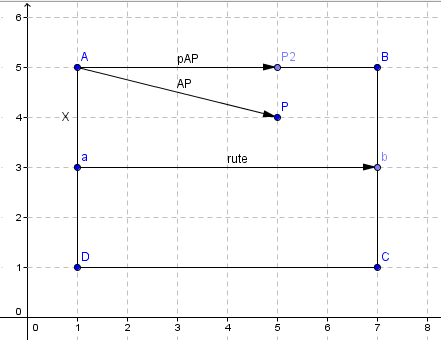
\includegraphics[scale=0.6]{matematikteori2} \newline
    \textit{Figur 5.2: Fortsat eksempel på om en attraktion er indenfor punkt a og b.}\newline
  \end{center}
  \vspace{-20pt}
\end{wrapfigure}

overholder punktet P første del, og ovenstående metode skal derfor gentages med vektoren AD i stedet for AB, for matematisk at finde ud af om punktet ligger inden 	for den afsatte bredde og længden af ruten a til b. Ved udregning af projektionen af AP på AD vil den nye vektor hedde: \[ \begin{bmatrix} 0 \\ -1 \end{bmatrix} \text{ .} \]\newline
\newline

\section{Implementering}
I dette afsnit vil programmet blive beskrevet, både en overordnet programbeskrivelse og en dybdegående forklaring af programmets funktioner. Derudover vil der blive beskrevet hvordan brugeren interagere med programmet. 

\subsection{Programbeskrivelse}
Programmet begynder med at indlæse alle de forudbestemte tilgængelige attraktioner fra en tekstfil. Alle disse attraktioner bliver vist på en liste for brugeren i kommandopromten med numre ud for hver attraktion. Brugeren vælger så hvilke attraktioner vedkommende har lyst til at besøge, ved at indtaste attraktionens nummer, hvor attraktionen så vil blive tilføjet til en liste. Denne liste kører gennem programmet, og den korteste rute bestemmes. Programmet tjekker derefter, for nærliggende attraktioner der kan tilføjes til ruten, på samme måde som i begyndelsen da de valgte attraktioner til deres rute. Hvis brugeren vælger ekstra attraktioner til deres rute, kører programmet igen, og den nye rute beregnes.  Når ruten er beregnet, vil ruten blive vist på skærmen, i den beregnede rækkefølge. Den samlede længde af ruten vil også blive vist.
\subsection{Beskrivelse af structs}
Til programmet bruges fire forskellige structs. Den første struct er "attraktion", som indeholder to strings, "navn" og "adresse", to doubles, "kmFraGreenwich" og "kmFraAekvator", og en int, "besoegt", der beskriver om attraktionen er besøgt eller ej. Denne struct bruges til at opdele og gamme de enkelte attraktioners data i programmet.\newline

\begin{lstlisting}
typedef struct {
	char navn[MAX_STRING];
	char adresse[MAX_STRING]; 
	double kmFraGreenwich, kmFraAekvator;
	int besoegt;
} attraktion;
\end{lstlisting} 

Næste struct er "naboRute", som indeholder en double, "ruteLaengde", og et array af attraktioner, "rute". Denne struct bruges til at lave ruter, hvor "rutelaengde" er længden af ruten og arrayet indeholder rækkefølgen af attraktioner på ruten. \newline

\begin{lstlisting}
typedef struct {
	double ruteLaengde;
	attraktion rute[ANTAL_ATTRAKTIONER];
} naboRute;
\end{lstlisting}

Næste struct er "kant", som indeholder to attraktioer, "startAttraktion" og "slutAttraktion", og en double, "laengde". Denne struct bliver brugt til at gemme data omkring afstanden mellem to punkter.\newline

\begin{lstlisting}
typedef struct {
  attraktion start;
  attraktion slut;
  double laengde;
} kant;
\end{lstlisting}

Sidste struct er "vektor", som indeholder to doubles, "x" og "y". Denne struct bruges til at gemme x og y koordinater for vektorer (og i nogle tilfælde punkter) under et navn. \newline

\begin{lstlisting}
typedef struct {
  double x, y;
} vektor;
\end{lstlisting}

\subsection{Beskrivelse af funktioner}
Attraktionerne til programmet bliver indlæst fra en .txt fil når prorammet køres. I programmet bliver filen indlæst i en funktion som hedder initialiserAttraktioner. Hvis filen ikke er tom vil elementerne, vha. funktionen fscanf, blive indlæst i grupper af 4, hvor de bliver indlæst som ”attraktion” hvilket er defineret som et struct. Hvis filen er tom, vil en advarsel blive vist i prompten og lukke programmet ned. Når alt information er indlæst fra filen, og den ikke længere er nødvendig, lukkes filen.\newline

\begin{lstlisting}
void initialiserAttraktioner(attraktion *attraktioner){
  FILE *input_file_pointer;
  int i = 0;
  double lndgrad;
  double brdgrad;

  input_file_pointer = fopen("attraktioner.txt", "r");

  if(input_file_pointer != NULL){
    while(fscanf(input_file_pointer, " %s %s %lf %lf", attraktioner[i].navn, attraktioner[i].adresse, &brdgrad, &lndgrad) == 4){
      attraktioner[i].kmFraGreenwich = lndgrad * KM_PR_LNDGRAD;
      attraktioner[i].kmFraAekvator = brdgrad * KM_PR_BRDGRAD;
      attraktioner[i].besoegt = 0;
      i++;
    }
  }else{
    printf("kunne ikke aabne fil\n"); exit(1);
  }
  fclose(input_file_pointer);
} 
\end{lstlisting}

Funktionen ”udregn\_kanter” bruges til at udregne distancen mellem punkterne. Beregningen af distancerne sker vha. ”beregn\_dist”, ved at sende en start og slut attraktion. Derefter bliver start- og slut attraktionen plus længden imellem dem lagt ind som en kant i kanter arrayet. Dette gøres i en for løkke i en anden for løkke, hvor der for hvert punkt blive udregnet distancen til de punkter der ikke allerede er blevet oprettet en kant for i en tidligere itteration af løkkerne. For hver kant der bliver oprettet, oprettes en ekstra kant som har samme længde, men har modsat start og slut attraktion. Så hvis det oprettes en kant fra x til y, vil der også blive oprettet en kant fra y til x med samme længde. Kanterne bliver tilføjet til kantarrayet, gennem den pointer der er inputparameter til funktionen, så kanterne kan blive tilgået fra resten af programmet. \newline

\begin{lstlisting}
void udregn_kanter(attraktion *attraktioner, kant *kanter)
{
	int i;
	int y;
	int indexTilKanter = 0;
	for (i = 0; i < ANTAL_ATTRAKTIONER; i++)
	{
		for (y = i; y < ANTAL_ATTRAKTIONER; y++)
		{
			if (strcmp(attraktioner[i].navn, attraktioner[y].navn) != 0)
			{
				kant k, j;
				k.start = attraktioner[i];
				j.slut = k.start;
				k.slut = attraktioner[y];
				j.start = k.slut;
				k.laengde = beregn_dist(k.start, k.slut);
				j.laengde = k.laengde;
				kanter[indexTilKanter] = k;
				kanter[indexTilKanter+1] = j;
				indexTilKanter += 2;
			}
		}
	}
}
\end{lstlisting}

Funktionen ”beregn\_dist” er en implementering af pythagoras's sætning til at finde længden imellem 2 punkter. Funktionen returnere den beregnede distance mellem de to attraktioner. \newline

\begin{lstlisting}
double beregn_dist(attraktion startAttraktion, attraktion slutAttraktion)
{
  return sqrt(pow(startAttraktion.kmFraGreenwich - slutAttraktion.kmFraGreenwich, 2) + 
          pow(startAttraktion.kmFraAekvator - slutAttraktion.kmFraAekvator, 2));
}
\end{lstlisting}

Brugeren bliver præsenteret for en liste over alle tilgængelige attraktioner fra inputparameteren, og attraktionernes tilhørende nummer i funktionen "valgafAttraktioner. Brugeren bliver bedt om at indtaste attraktionernes matchende numre, hvilket vil blive tilføket til en list. Taster brugeren 0, bliver brugeren præsentere for sine valg, og beregninger af den korteste rute igangsættes. Programmet returnere listan af valgte attraktioner. \newline

\begin{lstlisting}
void valgafAttraktioner(attraktion *attraktioner, attraktion *valgteAttraktioner, int *antalValgteAttraktioner, attraktion *ikkeValgteAttraktioner){
	int i = 0, j = 0, k = 0, l = 0, m = 0, n = 0, o = 0, valgt = 0;
	
	for(i = 0; i < ANTAL_ATTRAKTIONER; i++){
		printf("%d: %s\n", i+1, attraktioner[i].navn);
	}
	
	printf("vaelg de attraktioner du oensker at se ved at skrive det tilhoerende tal.\n");
	printf("vaelg et tal (svarende til en attraktion) af gangen og tryk enter efter hver indtastet tal\n");
	printf("indtast ikke samme tal 2 gange\n");
	do{
		if(scanf("%d", &k) != 1){
		printf("Fejl i indlaesning. Farvel.\n"); exit(0);
		}
		if(k != 0){
			valgteAttraktioner[j] = attraktioner[k-1];
			j++;
		}
	} while(j < ANTAL_ATTRAKTIONER && k != 0);
	
	for (l = 0; l < ANTAL_ATTRAKTIONER; ++l)
	{
		valgt = 0;
		for (m = 0; m < j; ++m)
		{
			if(strcmp(attraktioner[l].navn, valgteAttraktioner[m].navn) == 0){
				m = j;
				valgt = 1;
			}	
		}
		if(valgt != 1){
			ikkeValgteAttraktioner[n] = attraktioner[l];
			n++;
		}
	}
	*antalValgteAttraktioner = j;
}
\end{lstlisting}
	
Funktionen ”findNaboRute” benytter NNA (Nearest Neighbour Algorithm, eller Nærmeste Nabo Algoritme), til at finde den korteste rute mellem en række attraktioner for et bestemt startsted, der er opgivet i inputparametrene. Efter at have fundet den korteste rute ud fra NNA som en beskrevet i teoriafsnittet X, returnere den et array med ruten og distancen for denne rute. \newline

\begin{lstlisting}
void findNaboRute(attraktion *valgteAttraktioner, int antalValgteAttraktioner, attraktion *startAttraktion, kant *kanter, attraktion **tempRute, double *ruteLaengde){
	int i = 0;
	double lavesteLaengde = 10000;
	*ruteLaengde = 0;

	tempRute[i] = startAttraktion;

	for(i = 0; i < antalValgteAttraktioner-1; ++i){ /*da der f.eks. kun er 4 kanter imellem 5 punkter*/
		tempRute[i]->besoegt = 1;
		int j = 0;
		for (j = 0; j < antalValgteAttraktioner; ++j)
		{
			if(valgteAttraktioner[j].besoegt != 1 && findDist(*tempRute[i], valgteAttraktioner[j], kanter) < lavesteLaengde){
				lavesteLaengde = findDist(*tempRute[i], valgteAttraktioner[j], kanter);
				tempRute[i+1] = &valgteAttraktioner[j];
			}
		}
		*ruteLaengde += lavesteLaengde;
		lavesteLaengde = 10000;
	}
	tempRute[antalValgteAttraktioner] = startAttraktion;
	*ruteLaengde += findDist(*tempRute[antalValgteAttraktioner-1], *tempRute[antalValgteAttraktioner], kanter);
}
\end{lstlisting}

”findKortesteNaboRute” benytter funktionen ”findNaboRute”, til at finde ud af hvilket startsted der giver den korteste rute. Dette gøres ved at sætte en variable til en stor værdi, som rutedistancen ikke vil gå over, og opdatere den hvis ”findNaboRute” returnere en distance for ruten gennem de givne attraktioner med en given start attraktion, der er lavere end de forgående ruter. ”findKortesteNaboRute” returnere et array med en korteste rute, og den samlede længde af denne rute.  \newline

\begin{lstlisting}
void findKortesteNaboRute(attraktion *valgteAttraktioner, int antalValgteAttraktioner, attraktion *ruteAttraktioner, kant *kanter, double *samletLaengde){
	/* indput er valgteAttraktioner arrayet, og kanter arrayet*/
	/*output er ruteAttraktioner og samletLaengde*/
	double ruteLaengde;
	attraktion *tempRute[antalValgteAttraktioner+1];
	*samletLaengde = 100000;
	
	int i;
	int h;
	int j;
	for (i = 0; i < antalValgteAttraktioner; ++i)
	{
		for (h = 0; h < antalValgteAttraktioner; ++h)
		{
			valgteAttraktioner[h].besoegt = 0;
		}
		findNaboRute(valgteAttraktioner, antalValgteAttraktioner, &valgteAttraktioner[i], kanter, tempRute, &ruteLaengde);
		if(ruteLaengde < *samletLaengde){
			*samletLaengde = ruteLaengde;
			for (j = 0; j < antalValgteAttraktioner+1; ++j)
			{
				ruteAttraktioner[j] = *tempRute[j];
			}
		}
	}
}
\end{lstlisting}

Funktionen "findDist" gennemgår alle kanter der allerede er oprettet, og returnere distancen mellem to attraktioner, som er sendt med kaldet af funktionen, uden at skulle beregne den igen. \newline

\begin{lstlisting}
double findDist(attraktion start, attraktion slut, kant *kanter){
  int i;
  for (i = 0; i < ANTAL_KANTER; ++i)
  {
    if(strcmp(kanter[i].start.navn, start.navn) == 0 && strcmp(kanter[i].slut.navn, slut.navn) == 0){
      return kanter[i].laengde;
    }
  }
  printf("Kunne ikke finde passende kant\n"); exit(0);
}
\end{lstlisting}

Funktionen ”attraktionErTilfoejet” bruges til at finde ud af, om en attraktioner allerede er tilføjet til ens liste over ekstra attraktioner, og returnere enten true eller false. \newline

\begin{lstlisting}
int attraktionErTilfoejet(attraktion *ekstraAttraktioner, int antalEsktraAttraktioner, attraktion attraktionAtTilfoeje){
	int i;
	for (i = 0; i < antalEsktraAttraktioner; ++i)
	{
		if(strcmp(ekstraAttraktioner[i].navn, attraktionAtTilfoeje.navn) == 0){
			return 1;
		}
	}
	return 0;
}
\end{lstlisting}

Funktionen ”prikProdukt” bruges til at finde prikproduktet mellem to vektorer, hvilket også er det funktionen returnere. \newline

\begin{lstlisting}
double prikProdukt(vektor vektor1, vektor vektor2){
	return (vektor1.x * vektor2.x) + (vektor1.y * vektor2.y);
}
\end{lstlisting}

Funktionen ”findEkstraAttraktionerFirkant” benytter beregningerne fra teoriafsnittet "Vektorteori", til at finde ud af om der findes en evt. interessant attraktion på brugerens rute. Der tjekkes om attraktionAtTilfoeje ligger inden for en bestemt distance til linjen mellem start og slut punkter. Vis attraktionAtTilfoeje ligger indenfor, bliver den lagt i ekstraAttraktioner arrayet. \newline

\begin{lstlisting}
void findEkstraAttraktionerFirkant(attraktion startAttraktion, attraktion slutAttraktion, attraktion *valgteAttraktioner, 
int *antalValgteAttraktioner, kant *kanter, attraktion attraktionAtTilfoeje, double maxDist, 
attraktion *ekstraAttraktioner, int *antalEsktraAttraktioner){
	int i, j;
	double vektorLaengde;
	vektor ruteVektor, ruteVinkelretVektor, ruteEnhedsVinkelretVektor, mainHjoerne, side1Vektor, side2Vektor, punktVektor;
	
	vektorLaengde = findDist(startAttraktion, slutAttraktion, kanter);
	ruteVektor.x = slutAttraktion.kmFraGreenwich - startAttraktion.kmFraGreenwich;
	ruteVektor.y = slutAttraktion.kmFraAekvator - startAttraktion.kmFraAekvator;
	ruteVinkelretVektor.x = -ruteVektor.y;
	ruteVinkelretVektor.y = ruteVektor.x;
	ruteEnhedsVinkelretVektor.x = ruteVinkelretVektor.x / vektorLaengde;
	ruteEnhedsVinkelretVektor.y = ruteVinkelretVektor.y / vektorLaengde;
	mainHjoerne.x = startAttraktion.kmFraGreenwich + ruteEnhedsVinkelretVektor.x * maxDist;
	mainHjoerne.y = startAttraktion.kmFraAekvator + ruteEnhedsVinkelretVektor.y * maxDist;
	side1Vektor.x = ruteVektor.x;
	side1Vektor.y = ruteVektor.y;
	side2Vektor.x = -2 * ruteEnhedsVinkelretVektor.x * maxDist;
	side2Vektor.y = -2 * ruteEnhedsVinkelretVektor.y * maxDist;
	
	punktVektor.x = attraktionAtTilfoeje.kmFraGreenwich - mainHjoerne.x;
	punktVektor.y = attraktionAtTilfoeje.kmFraAekvator - mainHjoerne.y;
	if(0 < prikProdukt(punktVektor, side1Vektor) && prikProdukt(punktVektor, side1Vektor) < prikProdukt(side1Vektor, side1Vektor) &&
	0 < prikProdukt(punktVektor, side2Vektor) && prikProdukt(punktVektor, side2Vektor) < prikProdukt(side2Vektor, side2Vektor)){
		ekstraAttraktioner[*antalEsktraAttraktioner] = attraktionAtTilfoeje;
		*antalEsktraAttraktioner += 1;
	}
}
\end{lstlisting}

For at foreslå ekstra attraktioner til den valgte rute, bruges funktionen ”findEkstraAttraktioner”, hvor dette vil udgøre den interessante rute. Dette gøres den ved først at bruge funktionen ”findDist”, til at finde ikke valgte attraktioner inden for en bestemt distance af de valgte attraktioner. Er en attraktion ikke inden for denne radius, bruges funktionen ”findEkstraAttraktionerFirkant” for at finde ud af, om attraktionen ligger tæt på ruten mellem to attraktioner. De attraktioner der enten er inden for den bestemte distance af enten attraktionerne eller ruterne derimellem, tilføjes til et array der returneres fra funktionen. \newline

\begin{lstlisting}
void findEkstraAttraktioner(attraktion *ruteAttraktioner, attraktion *valgteAttraktioner, int *antalValgteAttraktioner, 
kant *kanter, attraktion *ikkeValgteAttraktioner, double maxDist, attraktion *ekstraAttraktioner, int *antalEsktraAttraktioner){
	
	int i, j, antalIkkeValgteAttraktioner = ANTAL_ATTRAKTIONER - *antalValgteAttraktioner;
	
	for (i = 0; i < *antalValgteAttraktioner; ++i)
	{
		for (j = 0; j < antalIkkeValgteAttraktioner; ++j)
		{
			
			if(attraktionErTilfoejet(ekstraAttraktioner, *antalEsktraAttraktioner, ikkeValgteAttraktioner[j])){
			}else if(findDist(ruteAttraktioner[i], ikkeValgteAttraktioner[j], kanter) < maxDist || 
			findDist(ruteAttraktioner[i+1], ikkeValgteAttraktioner[j], kanter) < maxDist){
				ekstraAttraktioner[*antalEsktraAttraktioner] = ikkeValgteAttraktioner[j];
				*antalEsktraAttraktioner += 1;
			}else{
				findEkstraAttraktionerFirkant(ruteAttraktioner[i], ruteAttraktioner[i+1], valgteAttraktioner, antalValgteAttraktioner,
			kanter, ikkeValgteAttraktioner[j], maxDist, ekstraAttraktioner, antalEsktraAttraktioner);
		}
	}
}
}
\end{lstlisting}

Funktionen ”aendre\_startsted”, tager en rute som inputparameter, sammen med det startsted der ønskes. Funktionen laver derefter et nyt array, der har det nye startsted som første og sidste element, så ruten starter i startstedet, og vender tilbage dertil. Dette array er hvad funktionen returnere.  \newline

\begin{lstlisting}
void aendre_startsted(attraktion *ruten, attraktion nytStartSted, int antalAttraktioner, attraktion *outputRute)
{
	int i = 0, startStedIndex = 0;
	
	for (i = 0; i < antalAttraktioner; i++)
	{
		if (strcmp(ruten[i].navn, nytStartSted.navn) == 0)
		startStedIndex = i;
	}
	
	for (i = 0; i < antalAttraktioner; i++)
	{
		
		if (startStedIndex == antalAttraktioner-1)
		{
			startStedIndex = 1;
			outputRute[i] = ruten[0];
		}
		else
		{
			outputRute[i] = ruten[startStedIndex];
			startStedIndex++;
		}
	}
}
\end{lstlisting}

\subsection{Flowcharts}
Til overstående funktioner er der lavet flowcharts, over programmets funktionalitet og udførelse, samt hvordan de arbejder sammen.\newline

\begin{wrapfigure}{r}{0.5\textwidth}
  \vspace{-40pt}
  \begin{center}
    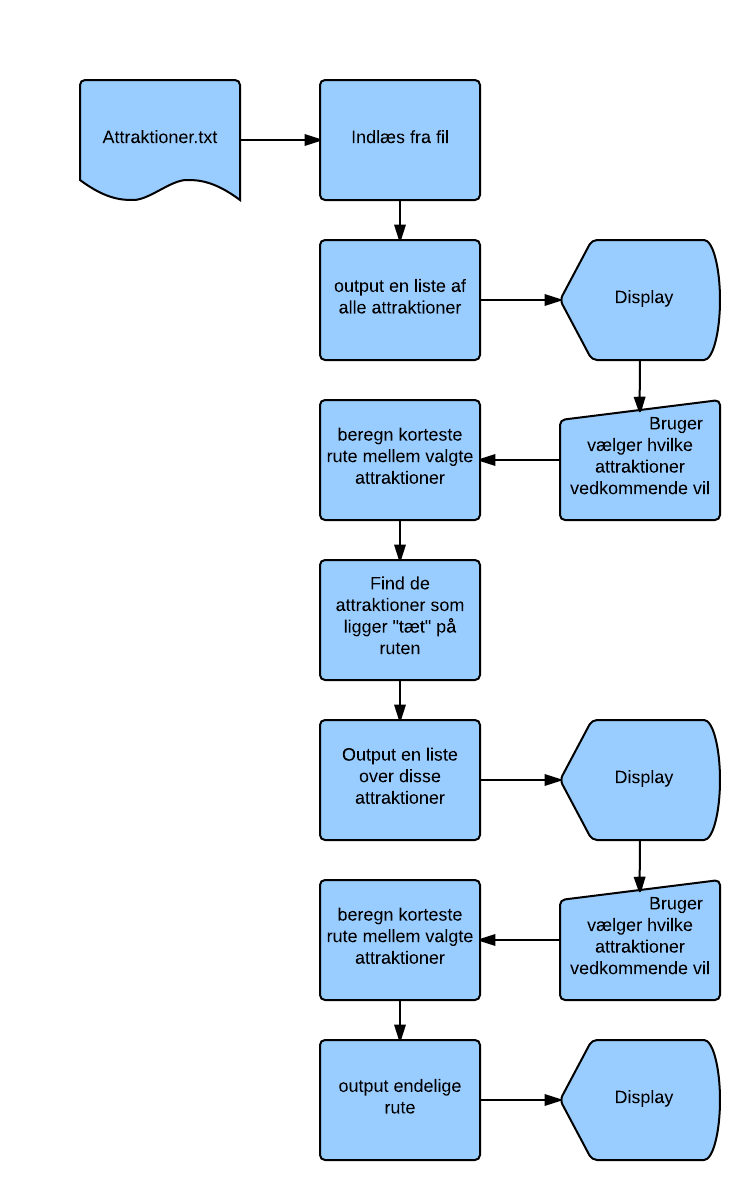
\includegraphics[scale=0.75]{program}\newline
    \textit{Figur 4.x: Rute - Ruten er hentet fra Maps.Google.com}
  \end{center}
  \vspace{0pt}
  \vspace{0pt}
\end{wrapfigure}

Der kommer flere flowcharts